%!TEX root = ../../main.tex

\chapter{Theoretical Background}
\section{RISC-V}
RISC-V is an open standard \acf{ISA} developed by the
University of California, Berkely. The ISA is based on reduced instruction set
computer (RISC) principles. The ISA supports 32, 64 and 128 bit architectures and
includes different extensions like Multiplication, Atomic, Floating Point and more. The
ISA is open source and therefore can be used by everyone without licensing issues
and high fee requirements. Due to the open source nature of the RISC-V project,
many companies like Alibaba and NVIDIA have started to develop hardware based
on this ISA.
RISC-V opens the opportunity to optimize and configure computer hardware to a
level that would not be realizable with licensed ISA like ARM or x86. As a result of
this possibility there are many projects and companies working on hardware and
software that are beating common CPU in terms of performance and power usage
by a lot.


\section{FPGA}
To verify a digital circuit software simulations as well as implementing the design on
a prototype are common practice. For prototyping and even implementing a finished
product, FPGA are widely used.
FPGAs are special fine granularity Programmable Logic Devices. The digital logic
can be described using hardware description languages such as Verilog or VHDL.
These designs are then synthesized, placed and routed in order to generate a
hardware configuration file, also called bitstream. The bitstream can then be loaded
onto the FPGA via a programming interface e.g. JTAG.
Many different vendors produce FPGAs, the most famous ones are Xilinx,
Altera/Intel and Microchip. Some smaller vendors like NanoXplore produce FPGAs
targeting rare use cases like space applications.
Despite the many differences in design of an FPGA, the basic architecture always
remains the same. An array of logic cells and building blocks of different features
9 like BRAM and DSP slices are connected to each other through configurable routing
channels.
Figure 2 shows the basic architecture of a Xilinx FPGA:\\

\begin{figure}[h]
\centering
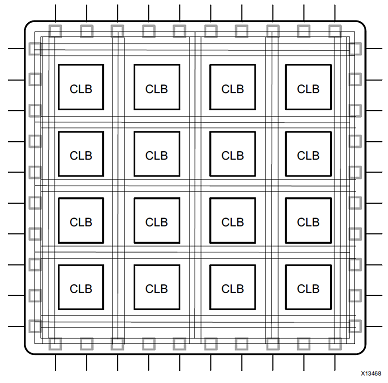
\includegraphics[scale=0.9]{fpga.png}
\caption{Xilinx FPGA\footnotemark}
\end{figure}



The CLBs in this architecture are comprised of LUTs and Flip-Flops, in order to implement boolean functions and allow the design of synchronous circuits. FPGAs produced by Xilinx are mostly SRAM based, other approaches are flash or anti-fuse based architectures.
\footnotetext{Source: \cite{xilinx:2017}}